\input{../preamble.tex}

\SetDate[11/03/2026]

\begin{document}
\pagestyle{fancy}
\fancyhead[L]{Première spécifique}
\fancyhead[C]{\textbf{Chapitre 7 — Dérivation}}
\fancyhead[R]{\today}

\newcommand{\hide}[1]{\phantom{#1}}
% (un)comment below for completion
% cannot renew phantom itself otherwise multicols environment shows a "p" in the right margin idk why
%\renewcommand{\hide}[1]{{\color{RED_E!80!BLACK}#1}}

\section{Fonctions affines}

\begin{figure}[h]
	\centering
%\def\arraystretch{2}
%\setlength\tabcolsep{10pt}
	\begin{tabular}{|c|c|c|c|c|c|c|c|}\hline
		$x$ & $-3$ & $-2$ & $-1$ & $0$ &  1 & 2 & 3 \\ \hline
		$f(x) = -2x+1$ & \hide{7} & \hide{5} & \hide{3} & \hide{1} & \hide{-1} & \hide{-3} & \hide{-5} \\ \hline
	\end{tabular}
	\caption{Tableau de valeurs de $f(x) = -2x+1$.}
	\label{fig:f(t)}
\end{figure}


\begin{multicols}{2}
\begin{definition*}
	Une fonction $f$ est \emph{affine} si elle s'écrit
		\[ f(x) = \hide{ax+b,} \]
	où $a$ est \hide{le coefficient directeur.}
	
	La courbe représentative de $f$ est une \hide{droite de pente $a$.}
\end{definition*}

	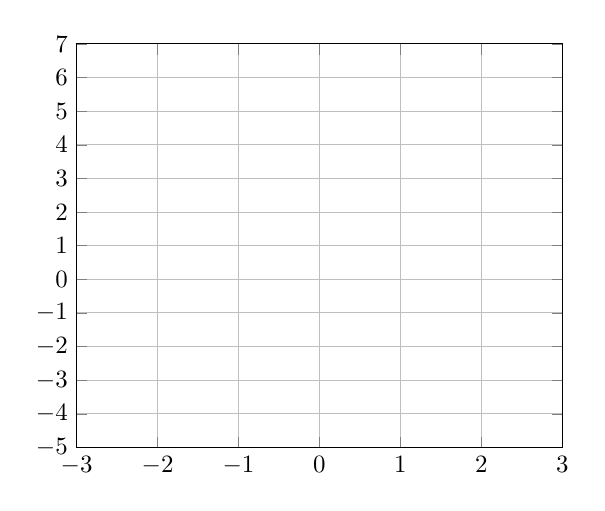
\begin{tikzpicture}[scale=.9]
	\begin{axis}[
	xmin = -3, xmax=3, ymin=-5, ymax=7, 
	grid = both,
	%label={$x$}, ylabel={$f(x) = -2x+1$},
	xtick distance = 1,
	ytick distance = 1,
	]
	%%%%%%%%%%%
	% (UN)COMMENT FOR SOLUTIONS
	%%%%%%%%%%%
	%\addplot[domain=-3:3, samples=2, BLUE_E, very thick]{2*x+1} node[pos=1, right]{$y=2x+1$};
	\end{axis}
	\end{tikzpicture}
\end{multicols}



\subsection{Coefficient directeur et variation}


\begin{theorem}
	Soient $f(x) = ax+b$ une fonction affine et $A(x_A ; y_A), B(x_B ; y_B)$ deux points appartenant à la droite $\C_f$.
	Alors
	\[ a = \hide{\dfrac{\text{différence des $y$}}{\text{différence des $x$}} = \dfrac{y_B - y_A}{x_B-x_A}.} \]
\end{theorem}

\begin{theorem}
	Soit $f$ une fonction affine et $a$ son coefficient directeur.
		\begin{enumerate}	
			\item si $a > 0$, alors $f$ est \hide{croissante sur $\R$.}
			\item si $a < 0$, alors $f$ est \hide{décroissante sur $\R$.}
			\item si $a = 0$, alors $f$ est \hide{constante sur $\R$.}
		\end{enumerate}
\end{theorem}


\subsection{Signe affine et signe de produit}

	Pour étudier le signe de $ax+b$, il faut
	\begin{enumerate}[label=\roman*), leftmargin=50pt]
		\item résoudre $ax+b = 0$ pour savoir en quel $x$ elle s'annule et l'ajouter au tableau ;
		\item reconnaitre si $ax+b$ est croissante, décroissante, ou constante ;
		\item en déduire le signe de $ax+b$ de part et d'autre du zéro à l'aide de ses variations.
	\end{enumerate}

\begin{exemple*}
	Étudions le signe du produit $(-2x+1)(3x+4)$.
	
	\hide{
	$-2x + 1 = 0 \iff x = \frac12$ et la fonction est décroissante car $-2<0$.
	%
	$3x + 4 = 0 \iff x = -\frac43$ et la fonction est croissante car $3>0$.
	%
	On place donc $\minfty, -\frac43, \frac12,$ et $\pinfty$ dans la ligne des $x$ importants, dans l'ordre croissant.
	%
	En remplissant le signe de chaque fonction affine, on déduit le signe du produit avec les règles usuelles $(-)\times(-) = (+)$, et $(-)\times(+) = (-)$, et $(+)\times(+) = (+)$.
	}
	
	\begin{center}
	\begin{tikzpicture}
		\tkzTabInit
		[lgt=4,]
       	{$x$ / 1, Signe de $-2x+1$ / 1, Signe de $3x+4$ / 1, Signe de $(-2x+1)(3x+4)$ / 1}
       	{\hide{$\minfty$},\hide{$-\frac43$},\hide{$\frac12$},\hide{$\pinfty$}}
		\hide{
		\tkzTabLine
       	{,-,,-,0,+,}
		\tkzTabLine
       	{,-,0,+,,+,}
		\tkzTabLine
       	{,+,0,-,0,+,}
		}
	\end{tikzpicture}
	\end{center}

\end{exemple*}

\section{Nombre dérivé}

\subsection{Vitesse instantanée}

\begin{exemple*}

On cherche à déterminer la vitesse d'une voiture au temps $t=1$ à l'aide des mesures suivantes.

\begin{center}
\begin{tabular}{|*{6}{c|}}\hline
	Temps (heure) & 0,9 & 1 & 1,2 & 1,5 & 2
	\\\hline
	Distance parcourue (km) & 9 & 10 & 12,2 & 16 & 23
	\\\hline
\end{tabular}
\end{center}

La formule de la vitesse est 
	\[ v = \hide{\dfrac{\text{différence de distance}}{\text{différence de temps}} = \dfrac{y_B-y_A}{x_B-x_A}.} \]

\begin{enumerate}[leftmargin=50pt]
	\item
	En utilisant $t=1$ et $t=2$, on obtient une vitesse de \hide{13 km/h.}
	
	\item
	En utilisant $t=1$ et $t=1,5$, on obtient une vitesse de \hide{12 km/h.}
	
	\item
	En utilisant $t=1$ et $t=1,2$, on obtient une vitesse de \hide{11 km/h.}
	
	\item
	En utilisant $t=1$ et $t=0,9$, on obtient une vitesse de \hide{10 km/h.}
	
\end{enumerate}

La vitesse instantanée de la voiture au temps $t=1$ est donc proche de \hide{10 km/h.}

\end{exemple*}

\subsection{Définition et propriétés}

%\begin{outil*}
%	Soient $x, y\in\R$ deux nombres distincts, et $f$ une fonction affine de coefficient directeur $a$.
%	Alors
%	
%\begin{multicols}{2}
%		%\[ a = \dfrac{f(y) - f(x)}{y-x}. \]
%		\[ a = \qquad\qquad\qquad \]
%		\vfill
%		\,
%		
%	\begin{tikzpicture}[scale=.8]
%	\begin{axis}[xmin = -2, xmax=2, ymin=-5, ymax=3, grid = none,  xlabel={$x$}, ylabel={$f(x)$}]
%		\addplot[domain=-2:2, samples=2, myb, thick] {2*x-1};
%		
%		\addplot[black, thick, mark=*, mark size = 1] (-1,-3) node[right=5pt] {$A(x; f(x))$};
%		\addplot[black, thick, mark=*, mark size = 1] (1,1) node[above left] {$B(y; f(y))$};
%	\end{axis}
%	\end{tikzpicture}
%\end{multicols}
%
%\end{outil*}



%\begin{exemple*}{étude de $\mathbf{f(x) = \dfrac12(x^3 + 2x^2 - x - 2)}$ autour de $\mathbf{x=-0,5}$}{}
%
%\begin{center}
%\begin{tikzpicture}[scale=.8]
%\begin{axis}[xmin = -3, xmax=2, ymin=-5, ymax=6, grid = none,  xlabel={$x$}, ylabel={$f(x)$}]
%	\addplot[domain=-3:2, samples=500, myb, thick] {.5*(x+2)*(x+1)*(x-1)};
%	
%	% zoom square A to B
%	\newcommand\xA{-2}
%	\newcommand\yA{-2}
%	\newcommand\xB{1}
%	\newcommand\yB{2}
%	\draw[black, thick] (axis cs:\xA,\yA) -- (axis cs:\xA,\yB);
%	\draw[black, thick] (axis cs:\xB,\yA) -- (axis cs:\xB, \yB);
%	\draw[black, thick] (axis cs:\xA,\yB) -- (axis cs:\xB,\yB);
%	\draw[black, thick] (axis cs:\xA,\yA) -- (axis cs:\xB,\yA);
%\end{axis}
%\end{tikzpicture}
%\begin{tikzpicture}[scale=.8]
%\begin{axis}[xmin = -2, xmax=1, ymin=-2, ymax=2, grid = none,  xlabel={$x$}, ylabel={$f(x)$}]
%	\addplot[domain=-2:1, samples=500, myb, thick] {.5*(x+2)*(x+1)*(x-1)};
%	
%	% zoom square A to B
%	\newcommand\xA{-1}
%	\newcommand\yA{-1.5}
%	\newcommand\xB{0}
%	\newcommand\yB{0.5}
%	\draw[black, thick] (axis cs:\xA,\yA) -- (axis cs:\xA,\yB);
%	\draw[black, thick] (axis cs:\xB,\yA) -- (axis cs:\xB, \yB);
%	\draw[black, thick] (axis cs:\xA,\yB) -- (axis cs:\xB,\yB);
%	\draw[black, thick] (axis cs:\xA,\yA) -- (axis cs:\xB,\yA);
%\end{axis}
%\end{tikzpicture}
%
%\begin{tikzpicture}[scale=.8]
%\begin{axis}[xmin = -1, xmax=0, ymin=-1.5, ymax=.5, grid = none,  xlabel={$x$}, ylabel={$f(x)$}]
%	\addplot[domain=-1:0, samples=500, myb, thick] {.5*(x+2)*(x+1)*(x-1)};
%	
%	% zoom square A to B
%	\newcommand\xA{-.75}
%	\newcommand\yA{-1}
%	\newcommand\xB{-.25}
%	\newcommand\yB{0}
%	\draw[black, thick] (axis cs:\xA,\yA) -- (axis cs:\xA,\yB);
%	\draw[black, thick] (axis cs:\xB,\yA) -- (axis cs:\xB, \yB);
%	\draw[black, thick] (axis cs:\xA,\yB) -- (axis cs:\xB,\yB);
%	\draw[black, thick] (axis cs:\xA,\yA) -- (axis cs:\xB,\yA);
%\end{axis}
%\end{tikzpicture}
%\begin{tikzpicture}[scale=.8]
%\begin{axis}[xmin = -.75, xmax=-.25, ymin=-1, ymax=0, grid = none,  xlabel={$x$}, ylabel={$f(x)$}]
%	\addplot[domain=-1:0, samples=500, myb, thick] {.5*(x+2)*(x+1)*(x-1)};
%	
%	\addplot[black, thick, mark=*, mark size = 1] (-.5,-.5625) node[right=5pt] {$A(x; f(x))$};
%	\addplot[black, thick, mark=*, mark size = 1] (-.6,-.448) ;
%	\addplot[black] (-.5,-.388) node{$B(x-h; f(x-h))$};
%	\addplot[black, thick, mark=*, mark size = 1] (-.4,-.672);
%	\addplot[black] (-.4,-.75) node{$C(x+h; f(x+h))$};
%\end{axis}
%\end{tikzpicture}
%\end{center}
%
%La pente de la droite $(AC)$ est
%	\[ a_h = \qquad\qquad\qquad\qquad\qquad\qquad. \]
%La pente de la droite $(AB)$ est
%	\[ a_h = \qquad\qquad\qquad\qquad\qquad\qquad. \]
%
%\end{exemple*}


%\begin{definition*}
%	On considère les coefficients directeurs
%		\begin{align*}
%			\dfrac{f(x+h) - f(x)}h, \label{eq:ah}
%		\end{align*}
%	où $h$ est de plus en plus petit.
%
%	Lorsque $h$ tend vers 0, on admet que qu'ils convergent vers une valeur qu'on note
%		\[ f'(x). \]
%	C'est le \emph{nombre dérivé} de $f$ en $x$.
%\end{definition*}

\begin{definition*}
	La droite approximant $\C_f$ localement autour de $x$ est la \hide{\quad tangente\quad} à $\C_f$ en $x$.
	Elle frôle $\C_f$ et son coefficient directeur est \hide{$f'(x)$.}
\end{definition*}

\begin{exemple*}
	Considérons la courbe de la fonction carré $f(x) = x^2$. Alors $f'(x) = \hide{2x.}$
	
	
	\begin{multicols}{2}
	\begin{tikzpicture}[scale=1]
	\begin{axis}[
		xmin = -3, 
		xmax=3, 
		ymin=0, 
		ymax=9, 
		clip=false, 
		minor tick num = 1,
		%extra x ticks={1.5},
		extra x ticks = {0},
		]
		\addplot[domain=-3:3, samples=500, BLUE_E, very thick]{x^2} node[pos=1, right]{$y=x^2$};
		
		% tangente x=0
		\addplot[domain=-.75:.75, samples=2, RED_E, very thick, <->] {0};
		% tangente x=1.5
		\addplot[domain=1:2, samples=2, RED_E, very thick, <->] {3*x-2.25};
		\addplot[densely dashed, BLACK, very thick] (1.5,0)--(axis cs:1.5,2.25);
		% tangente x=-2
		\addplot[domain=-2.5:-1.5, samples=2, RED_E, very thick, <->] {-4*x-4};
		\addplot[densely dashed, BLACK, very thick] (-2,0)--(axis cs:-2,4);
	\end{axis}
	\end{tikzpicture}
	%\columnbreak
	\null\vfill
\def\arraystretch{2}
\setlength\tabcolsep{10pt}
	\begin{tabular}{|*{6}{c|}}\hline
		$x$ & $-2$ & $1,5$ & 0 & 1,5 & 2 \\\hline
		$f'(x) = \hide{2x}$ & \hide{$-4$} & \hide{$-3$} & \hide{0} & \hide{3} & \hide{4}  \\\hline
	\end{tabular}
	\vfill\null
	\end{multicols}
	
\end{exemple*}



%\begin{exemple*}
%	On pose $x=-0,5$ et on prend $h$ de plus en plus petit dans l'équation \eqref{eq:ah} pour remplir le tableau figure \ref{fig:3}.
%	%\[ a_h = \dfrac{f(-0,5+h)-f(-0,5)}{h}. \]
%	\[ a_h = \hspace{5cm} \]
%	
%	On trace la droite de pente \hspace{2cm} passant par $(-0,5 ; f(-0,5))$ ci-dessous.
%\end{exemple*}
%
%\begin{figure}[h!]
%	\begin{subfigure}{0.18\textwidth}
%	\begin{tabular}{|c|c|}\hline
%		$h$ & $a_h$ \\ \hline
%		1 & \hspace{1cm} \\ \hline
%		0,1 & \\ \hline
%		0,001 & \\ \hline
%		-1 & \\ \hline
%		-0,1 & \\ \hline
%		-0,001 & \\ \hline
%	\end{tabular}
%	%\caption{Accroissements autour de $x=-0,5$.}
%	%\label{fig:3a}
%	\end{subfigure}
%	\hspace{5cm}
%	\begin{subfigure}{0.78\textwidth}
%	\begin{tikzpicture}[scale=1]
%	\begin{axis}[xmin = -3, xmax=2, ymin=-5, ymax=6, grid = none,  xlabel={$x$}, ylabel={$f(x)$}]
%		\addplot[domain=-3:2, samples=500, myb, thick] {.5*(x+2)*(x+1)*(x-1)};
%		
%		% tangente
%		\addplot[domain=-2:1, samples=2, myr, thick, <->] {-1.125*(x+.5)-.5625};
%	\end{axis}
%	\end{tikzpicture}
%	%\caption{Tangente à $\C_f$ en $x=-0,5$.}
%	%\label{fig:3b}
%	\end{subfigure}
%\caption{Calculs d'accroissements et tangente.}
%\label{fig:3}
%\end{figure}


%\begin{propriete}
%	$f'(x)$ est le coefficient directeur de la tangente à $f$ en $x$.
%\end{propriete}

\begin{theorem}
	Le signe de $f'(x)$ donne la variation de $f$ en $x$ et inversement :
		\begin{enumerate}
			\item si $f'(x) > 0$, alors \hide{$f$ est croissante autour de $x$.}
			\item si $f$ est croissante autour de $x$, alors \hide{$f'(x) > 0$.}
			\item si $f'(x) < 0$, alors \hide{$f$ est décroissante autour de $x$.}
			\item si $f$ est décroissante autour de $x$, alors \hide{$f'(x) < 0$.}
		\end{enumerate}
\end{theorem}


%\begin{exemple*}
%
%	\begin{center}
%	\begin{tikzpicture}
%		\tkzTabInit
%		 %[lgt=3,espcl=1.5]
%	       		{$x$ / 1 , Variation de $f(x)$ / 2, Signe de $f'(x)$ / 1}
%	       		{-3,,,,2}
%	\end{tikzpicture}
%	\end{center}
%\end{exemple*}

%\begin{strategie*}
%	On considère une courbe $\C_f$ lisse quelconque.
%	Par zooms successifs, on remarque que $\C_f$ devient presque droite.
%	L'erreur d'approximation devient de plus en plus petite en zoomant.
%	
%	\begin{enumerate}
%		\item On suppose $h$ assez petit tel que $\C_f$ soit droite sur $[x-h ; x+h]$.
%		\item On calcule le coefficient directeur de la droite à l'aide de l'équation \eqref{eq:ah}. Il tend vers $f'(x)$.
%		\item On regarde le signe de $f'(x)$ qui donne la variation de $f$ autour de $x$.
%	\end{enumerate}
%\end{strategie*}

\begin{corollaire}
	Un extremum local de $f$ survient lorsque $f$ change de \hide{variations.}

	Par conséquent, un extremum local de $f$ survient lorsque $f'$ change de \hide{signe.}
	
	Donc, si un extremum local de $f$ survient en $x$, on a nécessairement \hide{$f'(x) = 0$.}
\end{corollaire}
%\begin{strategie*}{déterminer les extrema de $f$}{}
%	\begin{enumerate}
%		\item On calcule $f'(x)$ comme précédemment.
%		\item On trouve les $x$ vérifiant $f'(x) = 0$.
%		\item On regarde le signe de $f'$ autour de $x$ : s'il change, c'est un extremum.
%	\end{enumerate}
%\end{strategie*}

\section{Étude de polynôme}

\begin{definition}
	Un \emph{polynôme} de degré 3 est une fonction de la forme
		\[ ax^3+ bx^2 + cx + d, \]
	avec $a, b, c, d$ des nombres appelés \emph{coefficients}.
\end{definition}

\begin{theorem}
	Soient $f, g$ deux fonctions dérivables, et $c\in\R$ un nombre réel quelconque. 
	Alors
		\vspace{-30pt}
		\begin{multicols}{2}
		\begin{enumerate}
			\item $(f+g)' = f' + g'$ %; et
			\item $(c \times f)' = c \times f'$.
		\end{enumerate}
		\end{multicols}
\end{theorem}


\begin{theorem}
	
	Pour chaque monôme suivant, on donne sa dérivée formelle.

\centering
\def\arraystretch{1.5}
%\setlength\tabcolsep{10pt}
	\begin{tabular}{|c|c|c|c|c|}\hline
		Monôme & 1 & $x$ & $x^2$ & $x^3$ \\ \hline
		Dérivée & \hide{0} & \hide{1} & \hide{$2x$} & \hide{$3x^2$} \\ \hline
	\end{tabular}
\end{theorem}

\begin{exemple*}
	Considérons la fonction $f(x) = 2x^3 - 6x + 3$ qu'on étudie pour $-2 \leq x \leq 2$.
	Pour quel(s) $x$ est-ce que $f(x)$ est maximale ? et minimale ?
	\begin{enumerate}
		\item
		La dérivée de $f$ est 
			\[ f'(x) = \hide{(2x^3 - 6x + 3)' = (2x^3)' - (6x)' + (3)' = 2\times3x^2 - 6 + 0 = 6x^2 - 6.}\]
		\item
		On montre que $f'(x) = 6(x-1)(x+1)$ en développant la forme factorisée donnée.
		\item
		On crée un tableau de signe de $f'(x)$ qu'on complète en un tableau de variations de $f(x)$.
	\end{enumerate}
	
	\begin{center}
	\begin{tikzpicture}
		\tkzTabInit
		 [lgt=3,espcl=4]
       	{$x$ / 1, Signe de $x+1$ / 1, Signe de $x-1$ / 1, Signe $f'(x)$ / 1, Variation de $f(x)$ / 2}
       	{\hide{$-2$},\hide{$-1$},\hide{1},\hide{2}}
		\hide{
		\tkzTabLine
       	{,-,0,+,,+,}
		\tkzTabLine
       	{,-,,-,0,+,}
		\tkzTabLine
       	{,+,0,-,0,+,}
		\tkzTabVar
			{-/$-1$,+/7,-/$-1$,+/7}
		}
	\end{tikzpicture}
	\end{center}

\end{exemple*}

\end{document}
